\section{Experiments}
\label{sec:experiment}
In this section, we conduct experiments on three real-world news datasets: 
Globo, Adressa and MIND. In order to simulate the real-time recommendation 
scenario, we use an offline evaluation method according to dates,  
which trains the model in the first few days and tests the trained model 
on the data for the next few days. We also set different scenarios 
to test the robustness of models. 

\subsection{Dataset and Setup}
\subsubsection{Dataset and preprocessing}
The Globo.com~\cite{moreira_news_2018} is the most popular news portal in Brazil, with numerous unique users and new contents per month. The dataset contains interaction sessions from Oct. 1 to 16, 2017, however, they didn't share the articles' textual content due to licensing reasons. Here, we use the trained article content embeddings provided by them. The three long-tail distribution of Globo is in \figref{fig:data_distribution}, 
which reveals the distinct characteristics of news reading: sessions are short, 
articles get outdated quickly and views are extremely sparse.
SmartMedia Adressa dataset~\cite{gulla_adressa_2017} is from a Norwegian news portal 
and it contains click events (including click time, 
clicked articles and active time period) 
and article content (including title and publish time) for three months. 
In our experiments, we use the first 20 days. If two successive click events point 
to the same articles, we merge them into one click event with active time added.
MIND~\cite{wu2020mind} is a large-scale news dataset collected from the Microsoft News website. It contains English news articles with rich textual content and impression logs of a week. Each impression log contains the click events as well as non-click events, and we construct user session according to each log. We crawl and fetch missing publish time of articles from given URL links.

\begin{figure}[th]
  \centering
  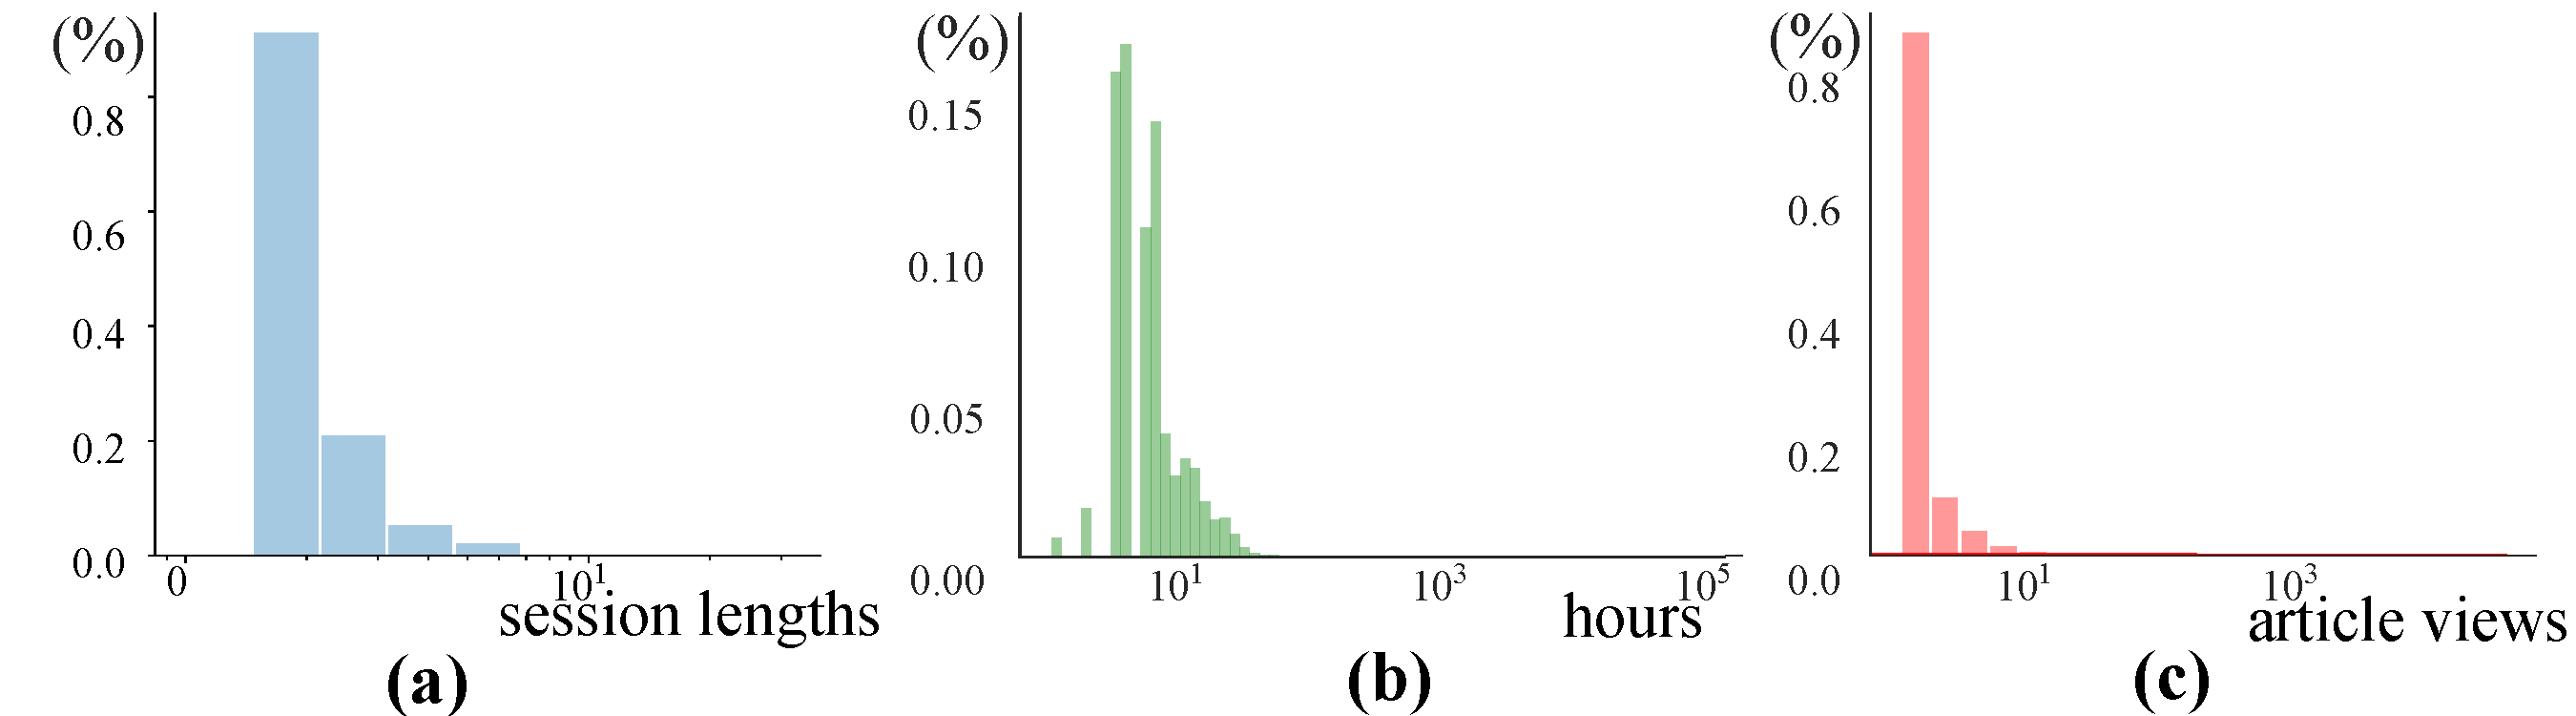
\includegraphics[width=\columnwidth]{fig/data_distribution.pdf}
  \caption{Distribution of session lengths, article ``freshness'' 
(click time $-$ article publish time), and \# of clicks per article.}
  \label{fig:data_distribution}
\end{figure}

\tabref{tb:dataset_info} lists the explicit information provided by these datasets. If the information is missing, we restore them with the implicit information. For the active time, we use the interval between two consecutive click time points, while for the impression list, we reconstruct it with articles near the time of publication.
\begin{table}[th]\setlength{\tabcolsep}{3pt}
  \caption{Explicit information (with $\checkmark$) provided by datasets}
  \label{tb:dataset_info}
  \centering
  \begin{tabular}{l|ccccc}
    \toprule
    % \multicolumn{2}{c}{Part}                   \\
    % \cmidrule(r){1-2}
     Dataset & \tabincell{c}{news\\content} & \tabincell{c}{temporal\\information} & \tabincell{c}{active\\time}  & \tabincell{c}{article\\impressions}\\
    \midrule
    Globo   & embeddings   & $\checkmark$ & from $tc$  & from $tp$  \\
    Adressa & $\checkmark$ & $\checkmark$ & $\checkmark$ & from $tp$\\
    MIND    & $\checkmark$ & partially & None & $\checkmark$ \\
    \bottomrule
  \end{tabular}
\end{table}

In dataset preprocessing, we treat a series of click events from one anonymous user 
within 30 minutes as a session, and a click event where click time is ahead of the 
article's publish time is regarded as a wrong sample and is discarded. 
We then filter out the sessions whose length is less than or equal to 1, 
to make sure that the model can give predictions based on at least one past click in
the same session. 
Because training data is limited, to augment it, 
we create mini-sessions whose start is the first click of the original
session and the ending is every other click in the session than the first.
Effectively, for a session of length $n$, we can create $n-1$ mini-sessions.
If a session in the test set only contains new articles that are not seen 
in the training set, we regard this session as a \textit{article cold-start} session, 
and the article cold-start ratio is computed as the percentage of such article cold-start sessions
over all sessions in the test set. The dataset statistics are 
in \tabref{tb:dataset}, and we can see that each session is quite short and 
more or less suffers from article cold-start problem.

\begin{table}[th]\setlength{\tabcolsep}{2.5pt}
  \caption{Dataset statistics (after preprocessing)}
  \label{tb:dataset}
  \centering
  \begin{tabular}{l|ccccccc}
    \toprule
    % \multicolumn{2}{c}{Part}                   \\
    % \cmidrule(r){1-2}
     Dataset & \tabincell{c}{\# sessions} & \tabincell{c}{\# articles} & \tabincell{c}{clicks\\/session}  & \tabincell{c}{clicks\\/article} & \tabincell{c}{Cold\\start} & \tabincell{c}{Days\\covered}\\
    \midrule
    Globo & 1M & 45k & 2.69 & 64 & 66.7\% & 16 \\
    Adressa & 0.5M & 12k & 2.78 & 116 & 70.9\% & 20 \\
    MIND & 0.2M & 7k & 2.38 & 59 & 60.3\% & 7 \\
    \bottomrule
  \end{tabular}
\end{table}

\subsubsection{Train/test set split}
In order to make our evaluations as realistic as possible, we do not adopt
the usual random train-test splits and cross-validation in this section. 
We follow the evaluation protocol by \citet{jugovac_streamingrec:_2018} to 
split the dataset by time, which trains the model with user sessions in the 
first few days and tests the trained model in the next few days. 
\figref{fig:data_split} shows how we create the train/test data.
%for Globo dataset, we split every 4 days into one fold, with 3 day for training and 1 day for testing, and 4 folds in total. For Adressa dataset, we split every 10 days into one fold due to its fewer session data in one day. We average metrics performance of each folds in the end. For MIND dataset, we leave the last day as test. 
After data augmentation, 
the ratio between training data and test data 
is around 6:1 for Globo, and 10:1 for the other two datasets. In Globo, we also split train/test set with the increasing number of training days 
and with the same training days but different days apart from the test day. 

\begin{figure}[th]
  \centering
  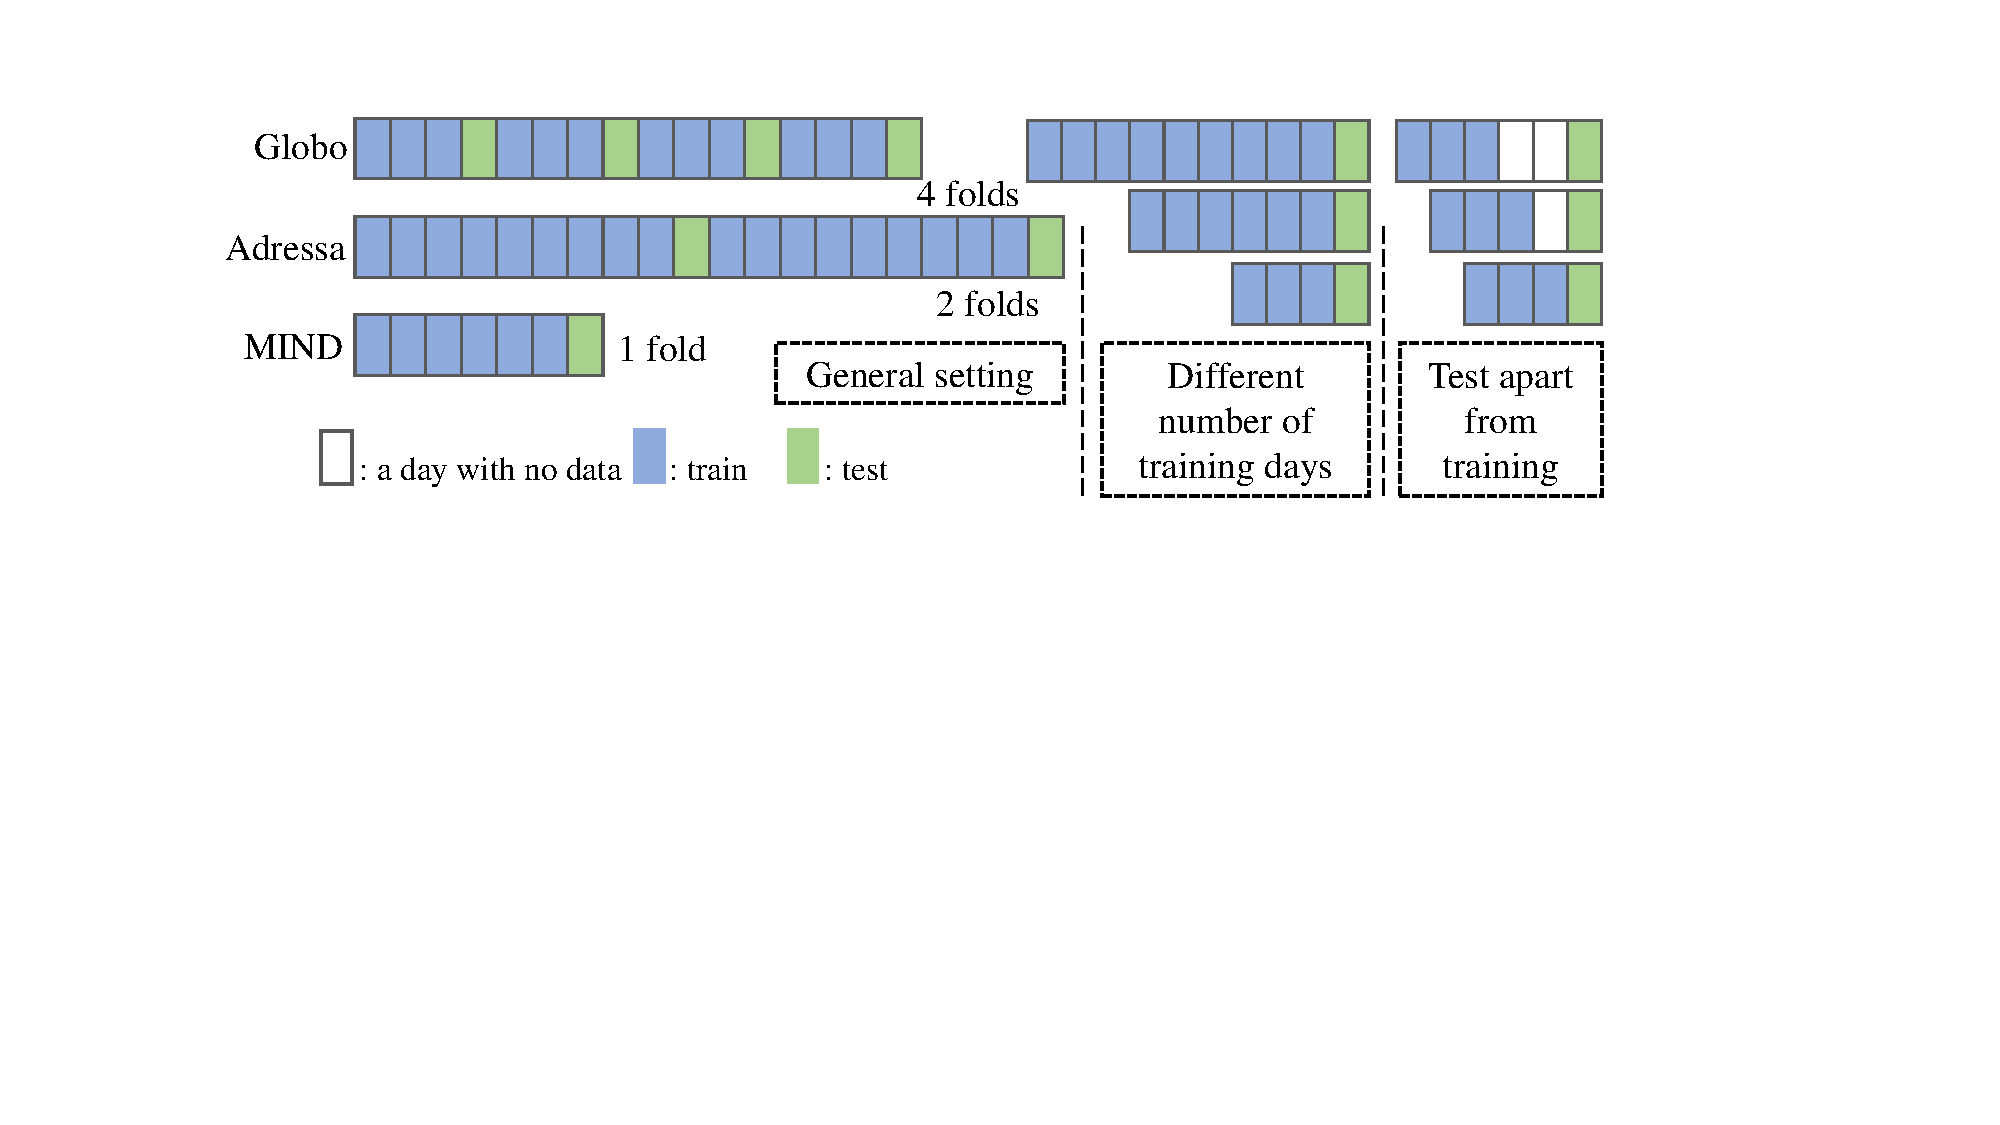
\includegraphics[width=\columnwidth]{fig/data_split.pdf}
  \caption{Dataset splits to simulate different scenarios.}
  \label{fig:data_split}
  \Description[Data split]{An illustration of train/test set split.}
\end{figure}

\subsubsection{Metrics}
During the test, given the first few click events in a session, the model will generate a recommendation list with probability from high to low. For $i$-th test sample ($N$ samples in total), we denote $p_i$ as the position of next clicked article $n_i$ in our prediction list $R_i$, and we use widely-used metrics HR@k (hit rate), NDCG@k (normalized discounted cumulative gain) to indicate the ability of the model to predict correct articles. 
\begin{equation}
  \begin{split}
    HR@k &= \frac{1}{N}\sum_{i\in N}\mathbbm{1}(p_i\leq k), \\
    NDCG@k &= \frac{1}{N}\sum_{i\in N}\frac{\mathbbm{1}(p_i\leq k)}{log_2(p_i+1)}, 
  \end{split}  
\end{equation}

Diversity represents the variety of items in recommendation lists, and reflects the model's
ability to recommend different items to different users. 
We define DR@k (diversity rate) as:
%of top-k prediction with real click data as normalization. 
%The larger DR refers that the model tends to recommend various articles to user.
\begin{equation}
  DR@k = \frac{|\{R_i[:k]\}_{i\in N}|}{|\{n_i\}_{i\in N}|},
\end{equation}
where $\{\cdot\}$ represents the union set.
\subsection{Baseline Algorithms}
%For this experiments, an extensive number of session-based recommendation algorithms was used for comparison, sequential modeling algorithms to predict next clicked item are also taken into consideration. Despite of the simplicity of some of those methods, they still have competitive accuracy on session-based recommendations.

\paragraph{Simple approaches without deep learning.}
\begin{itemize}
  \item CBCF~\cite{sottocornola2018session}, a news recommender combines Content-Based similarity with session-based Collaborative Filtering similarity. In experiments, we choose the best weighting factors for CB similarity and CF similarity in the experiment. We also list the results of separate CB and CF as a reference.
  \item STAN~\cite{garg2019sequence}, an extended version of SKNN (Session-KNN) with three controllable temporal decay factors. We choose hyperparameters suggested in their paper.
\end{itemize}

\paragraph{SOTA sequential recommendation approaches with deep learning.}
\begin{itemize}
  \item GRU4Rec~\cite{hidasi2015session,hidasi2018recurrent}, a Gated Recurrent Unit for recommendation, building with gated recurrent neural networks. We use backpropagation through time (BPTT), which usually performs better than the original GRU4Rec.
  \item SASRec~\cite{kang_self-attentive_2018}, a Self-Attention based Sequential model, adopting Transformer architecture to model user's action. We adopt cross-entropy as loss for better performance.
  \item STAMP~\cite{liu2018stamp}, a Short-Term Attention/Memory Priority Model for Session-based Recommendation, introducing attention mechanism to model the relationship of each historical click and the last click. We initialize the item embeddings with items' content vector.
  \item SR-GNN~\cite{wu2019session}, a Session-based Recommender using Graph Neural Networks to capture complex transitions of items.
\end{itemize}

\subsection{Implement Details}
For fair comparison, we apply the same augmented data except for CBCF, implement all methods in $TensorFlow$, and train models with Adam optimizer on one GTX1080Ti GPU. We use the same latent dimensions $d=250$ and choose different learning rate $\{0.01, 0.001, 0.0001\}$, batch size $\{512, 1024, 2048\}$ and other hyper-parameters to select the best model using early stopping strategy based on the HR@20 score on the validation set, which is the last 10\% samples in training set sorted by time. All embedding tables and weighting parameters are normally initialized with 0 mean, 0.002 and 0.05 standard deviation respectively.

\subsection{Main Results}
\label{sec:mainres}
\begin{table*}[th]\setlength{\tabcolsep}{2pt}
\caption{Main results ($k=20$). All results are averaged over all folds. 
* means attention-based methods. Best baseline result on each metric is underlined and 
overall best results are bolded.}
  \label{performance-table}
  \begin{threeparttable}
  \centering
  % \begin{tabular}{c|c|p{1.5cm}<{\centering}|c|c|p{1.5cm}<{\centering}|c|c|p{1.5cm}<{\centering}|c|c|p{1.5cm}<{\centering}|c}
  \begin{tabular}{p{1.4cm}<{\centering}|p{1.2cm}<{\centering}|p{1.2cm}<{\centering}|p{1.2cm}<{\centering}|p{1.2cm}<{\centering}|p{1.2cm}<{\centering}|p{1.2cm}<{\centering}|p{1.2cm}<{\centering}|p{1.2cm}<{\centering}|p{1.2cm}<{\centering}|p{1.2cm}<{\centering}|p{1.2cm}<{\centering}|p{1.2cm}<{\centering}}
  \toprule
  \multirow{2}{*}{Methods} & \multicolumn{3}{c|}{Globo} & \multicolumn{3}{c|}{Adressa} & \multicolumn{3}{c|}{MIND} & \multicolumn{3}{c}{Information} \\ 
  \cline{2-13} 
  & HR & NDCG & DR & HR & NDCG & DR & HR & NDCG & DR & Content & Session & Time \\ 
  \midrule
  CB    &3.55&1.37&\uline{4.40}&0.70&0.24&4.62&1.26&0.42&3.79&$\checkmark$&     &   \\
  CF    &11.05&4.37&1.77&9.24&3.29&2.49&2.48&0.88&2.22&     &$\checkmark$&   \\
  CBCF  &11.85&4.47&4.37&9.57&3.41&\uline{4.80}&3.15&1.10&\uline{4.06}&$\checkmark$&$\checkmark$&   \\
  STAN  &12.73&\uline{6.47}&0.98&11.30&5.00&1.21&3.12&1.42&1.09&     &$\checkmark$&$\checkmark$\\ 
  \midrule
  GRU4Rec&12.80&5.99&0.35&11.20&5.11&1.98&3.38&1.32&1.32&     &$\checkmark$&   \\
  SASRec$^*$ &\uline{14.09}&6.20&0.90&\uline{12.05}&5.09&1.37&\uline{3.55}&1.39&0.90&     &$\checkmark$&   \\
  SR-GNN &12.64&6.27&0.68&11.52&\uline{5.36}&2.29&3.34&\uline{1.44}&0.55&     &$\checkmark$&   \\
  STAMP$^*$ &12.47&5.94&0.63&12.01&5.28&1.62&3.31&1.25&1.22&     &$\checkmark$&   \\
  \midrule
  ITCAR$^*$ &\textbf{17.87}&\textbf{8.69}&\textbf{1.48}&\textbf{15.21}&\textbf{6.66}& 1.23 &\textbf{4.32}&\textbf{1.96} & 1.03&$\checkmark$&$\checkmark$&$\checkmark$\\ 
  \bottomrule
\end{tabular}
% \begin{tablenotes}
%   \item { }
% \end{tablenotes}
\end{threeparttable}
\end{table*}

%\tabref{performance-table} compares the end-to-end results of all methds. 
%Containing session information means the model utilizes the co-occurrence of articles in different sessions. 

In \tabref{performance-table}, we compare the performance of all baselines and our
approach, and we can make the following observations.

We first focus on traditional methods. CF captures the simplest co-occurrence patterns of articles but is quite effective already. CB gives low accuracy but yields high 
diversity, and boosts the results from CF to CBCF. This shows diverse content information can help explore fresh articles. CBCF is a typical example at the bottom right corner of the accuracy-diverse trade-off curve and we ignore the DR@20 of it in the later comparison. STAN makes use of temporal information, considering the recency of a past session, and the results are comparable to deep learning methods in three datasets even without content information. This shows the importance of temporal information in session-based recommendation. 

Next, we move to deep learning methods. SASRec beats others on HR@20 but is not so good in diversity. This reminds us of the dilemma between diversity and accuracy. Besides, we notice SR-GNN has a higher NDCG@20 score than other deep learning methods but the HR@20 is not always good, which means SR-GNN recommends target articles in higher ranking.

Finally, ITCAR performs significantly and consistently better than other methods in all the datasets on accuracy and for diversity the results are also competitive. 
Compared with deep learning methods, ITCAR not only model relations between articles but also integrates the user's different attention towards articles. Compared with CBCF and STAN, ITCAR is able to fuse content and temporal information of click event into session representation. It's usually a trade-off between accuracy and diversity for all kinds of recommendation systems, however, ITCAR mitigates this dilemma especially in the Globo dataset, where both recommendation quality and diversity are improved. While in other datasets the diversity is less good but still acceptable. We will give detailed analyses on different components of ITCAR in the ablation test (\secref{sec:abla}) and discussion (\secref{sec:discuss}).

In the MIND dataset, the HR/NDCG improvement is comparatively small. 
The possible reasons are: 
on the one hand, MIND didn't provide active interval, nor did they give click time of each article, we cannot get the positive feedback from the data; on the other hand, from the results of CBCF, we assume the article relational information is too sparse and thus hard to recommend. Noted that this dataset is not specially for the session-based recommendation, information may be lost through preprocessing.

\subsection{Ablation Studies}
\label{sec:abla}
To verify the effects of modeling user positive/negative implicit feedback as well as infusing temporal/content information addressed in ITCAR, we compare ITCAR with several variants to demonstrate the efficacy of the usage of positive implicit feedback behind active time, the temporal information of click time and publish time, the choice of negative samples. We set content-aware session representation as the baseline of the table. The results are shown in \tabref{tb:ablation}. Since there is no positive feedback in MIND, we use a 
constant value as a substitute. Here are the main findings. 

First, the effectiveness of positive implicit feedback can be verified according to (a) and (b), (f) and (g). With the active interval as implicit positive feedback, we gain a certain increase in both HR@20 and NDCG@20 than the plain content structure. Even though active interval is not explicitly offered in Globo, the interval between to consecutive clicks turns out to be useful. ITCAR loses the improvement in MIND due to the lack of this information. Also, from (f), removing positive signal impairs the final results.

Second, the temporal information plays a significant role in the full model. Although modeling session start time doesn't give remarkable advancement in accuracy, it makes up for the sacrifice of stage (b) in DR@20. As for modeling publish time of article sequence, it brings the greatest performance enhancement among all datasets, which indicates the importance of temporal information behind session interactions. 

Third, the negative samples from the impression list could provide complementary information that helps to learn user unbiased preferences. The random sampling strategy (e) worsens the performance, and this is presumably because it introduces noise and confuses the model, while (g) raises the scores in three datasets. This confirms our previous assumption about establishing impression lists according to publish time.

% \begin{table*}[!htp]\setlength{\tabcolsep}{1.5pt}
%   \caption{Ablation results ($k=20$). All results are averaged over all folds. 
% Cont: item and content embeddings only; Pos: with positive implicit feedback; Sta: with start time; Pub: with publish time as temporal info; Ran: random negative sampling; 
% Neg: with negative implicit feedback. (a) is the full model. $\Delta$ is the difference of HR@20 with (a)}
%   \label{tb:ablation}
%   \begin{threeparttable}
%   \centering
%   % \begin{tabular}{c|c|p{1.5cm}<{\centering}|c|c|p{1.5cm}<{\centering}|c|c|p{1.5cm}<{\centering}|c|c|p{1.5cm}<{\centering}|c}
%   \begin{tabular}{p{3.3cm}|p{1.1cm}<{\centering}|p{1.1cm}<{\centering}|p{1.1cm}<{\centering}|p{1.1cm}<{\centering}|p{1.1cm}<{\centering}|p{1.1cm}<{\centering}|p{1.1cm}<{\centering}|p{1.1cm}<{\centering}|p{1.1cm}<{\centering}|p{1.1cm}<{\centering}|p{1.1cm}<{\centering}|p{1.1cm}<{\centering}}
%   \toprule
%   \multirow{2}{*}{Variants} & \multicolumn{4}{c|}{Globo} & \multicolumn{4}{c|}{Adressa} & \multicolumn{4}{c}{MIND} \\ 
%   \cline{2-13} 
%   & HR & NDCG & DR & $\Delta$ & HR & NDCG & DR & $\Delta$ & HR & NDCG & DR & $\Delta$ \\ 
%   \midrule
%   (a) Full & 17.87 & 8.69 & 1.48 & - & 15.21 & 6.66 & 1.23 & - & 4.32 & 1.96 & 1.03 & - \\ 
%   (b) Full-Pos & 17.25 & 8.51 & 1.32 & -0.62 & 15.15 & 6.59 & 1.27 & -0.06  & - & - & - & -\\ 
%   (c) Full-Neg & 17.39 & 8.80 & 1.38 & -0.48 & 14.43 & 6.40 & 1.02 & -0.78 & 4.19 & 1.81 & 0.98 & -0.13\\
%   (d) Full-Neg+Ran & 17.22 & 8.38 & 1.35 & -0.65 & 14.36 & 6.39 & 1.30 & -0.85 & 4.06 & 1.71 & 0.81 & -0.26\\
%   (e) Full-Neg-Time & 13.45 & 6.55 & 1.16 & -4.42 & 12.54 & 5.60 & 0.87 & -2.67 & 3.66 & 1.65 & 0.60 & -0.66\\
%   % \midrule
%   \bottomrule
% \end{tabular}
% % \begin{tablenotes}
% %   \item { .}
% % \end{tablenotes}
% \end{threeparttable}
% \end{table*}


\begin{table*}[!htp]\setlength{\tabcolsep}{0.8pt}
  \caption{Ablation results ($k=20$). All results are averaged over all folds.
Cont: item and content embeddings only; Pos: with positive implicit feedback; Sta: with start time; Pub: with publish time as temporal info; Ran: random negative sampling;
Neg: with negative implicit feedback. (g) is the full model. $\Delta$ is the difference of HR@20 with (a)}
  \label{tb:ablation}
  \begin{threeparttable}
  \centering
  % \begin{tabular}{c|c|p{1.5cm}<{\centering}|c|c|p{1.5cm}<{\centering}|c|c|p{1.5cm}<{\centering}|c|c|p{1.5cm}<{\centering}|c}
  \begin{tabular}{p{3.7cm}|p{1.1cm}<{\centering}|p{1.1cm}<{\centering}|p{1.1cm}<{\centering}|p{1.1cm}<{\centering}|p{1.1cm}<{\centering}|p{1.1cm}<{\centering}|p{1.1cm}<{\centering}|p{1.1cm}<{\centering}|p{1.1cm}<{\centering}|p{1.1cm}<{\centering}|p{1.1cm}<{\centering}|p{1.1cm}<{\centering}}
  \toprule
  \multirow{2}{*}{Variants} & \multicolumn{4}{c|}{Globo} & \multicolumn{4}{c|}{Adressa} & \multicolumn{4}{c}{MIND} \\
  \cline{2-13}
  & HR & NDCG & DR & $\Delta$ & HR & NDCG & DR & $\Delta$ & HR & NDCG & DR & $\Delta$ \\
  \midrule
  (a) Cont (baseline) & 12.49 & 6.05 & 1.38 & - & 11.58 & 5.09 & 1.03 & - & 3.62 & 1.51 & 0.45 & -\\
  (b) Cont+Pos & 13.54 & 6.69 & 1.00 & \uline{1.05} & 12.50 & 5.62 & 0.57 & \uline{0.92} & - & - & - & - \\
  (c) Cont+Pos+Sta & 13.45 & 6.55 & 1.16 & 0.96 & 12.54 & 5.60 & 0.87 & 0.96 & 3.66 & 1.65 & 0.60 & 0.04\\
  (d) Cont+Pos+Sta+Pub & 17.39 & 8.80 & 1.38 & \uline{4.90} & 14.43 & 6.40 & 1.02 & \uline{2.85} & 4.19 & 1.81 & 0.98 & \uline{0.57}\\
  (e) Cont+Pos+Sta+Pub+Ran & 17.22 & 8.38 & 1.35 & 4.73 & 14.36 & 6.39 & 1.30 & 2.78 & 4.06 & 1.71 & 0.81 & 0.44\\
  \midrule
  (f) Cont+Sta+Pub+Neg & 17.25 & 8.51 & 1.32 & 4.76 & 15.15 & 6.59 & 1.27 & 3.57 & 4.32 & 1.96 & 1.03 & \uline{0.70} \\
  (g) Cont+Pos+Sta+Pub+Neg & 17.87 & 8.69 & 1.48 & \uline{5.38} & 15.21 & 6.66 & 1.23 & \uline{3.63} & - & - & - & - \\
  \bottomrule
\end{tabular}
% \begin{tablenotes}
%   \item { .}
% \end{tablenotes}
\end{threeparttable}
\end{table*}

\subsection{Discussion}
\label{sec:discuss}
We present some discussion on (i) the performance on user cold-start; 
(ii) the performance on article cold-start; (iii) the effect of the length of
training days and the gap between training days test days on the results; and 
(iv) A verification about the assumption of generating impression lists.
% \tabref{tb:cold}

\subsubsection{User cold-start}
\label{sec:usercold}
Since anonymous news sessions are short with average length of less than 3, 
the user cold-start problem is severe. We show the results for different input lengths in 
\figref{fig:inputlen}. Interestingly, ITCAR reaches its peak accuracy from length 1 to 2. 
In contrast, other methods all reach the peak at 3. 
Although STAN and CBCF use content and temporal information, 
they are inferior to ITCAR given the shorter input length. 
This shows ITCAR is capable of capturing user interests earlier in the session 
by leveraging user's implicit feedback. For longer input length, 
the difference between ITCAR and others narrows, 
indicating similar ability to predict given longer history. 

\begin{figure}[th]
  \centering
  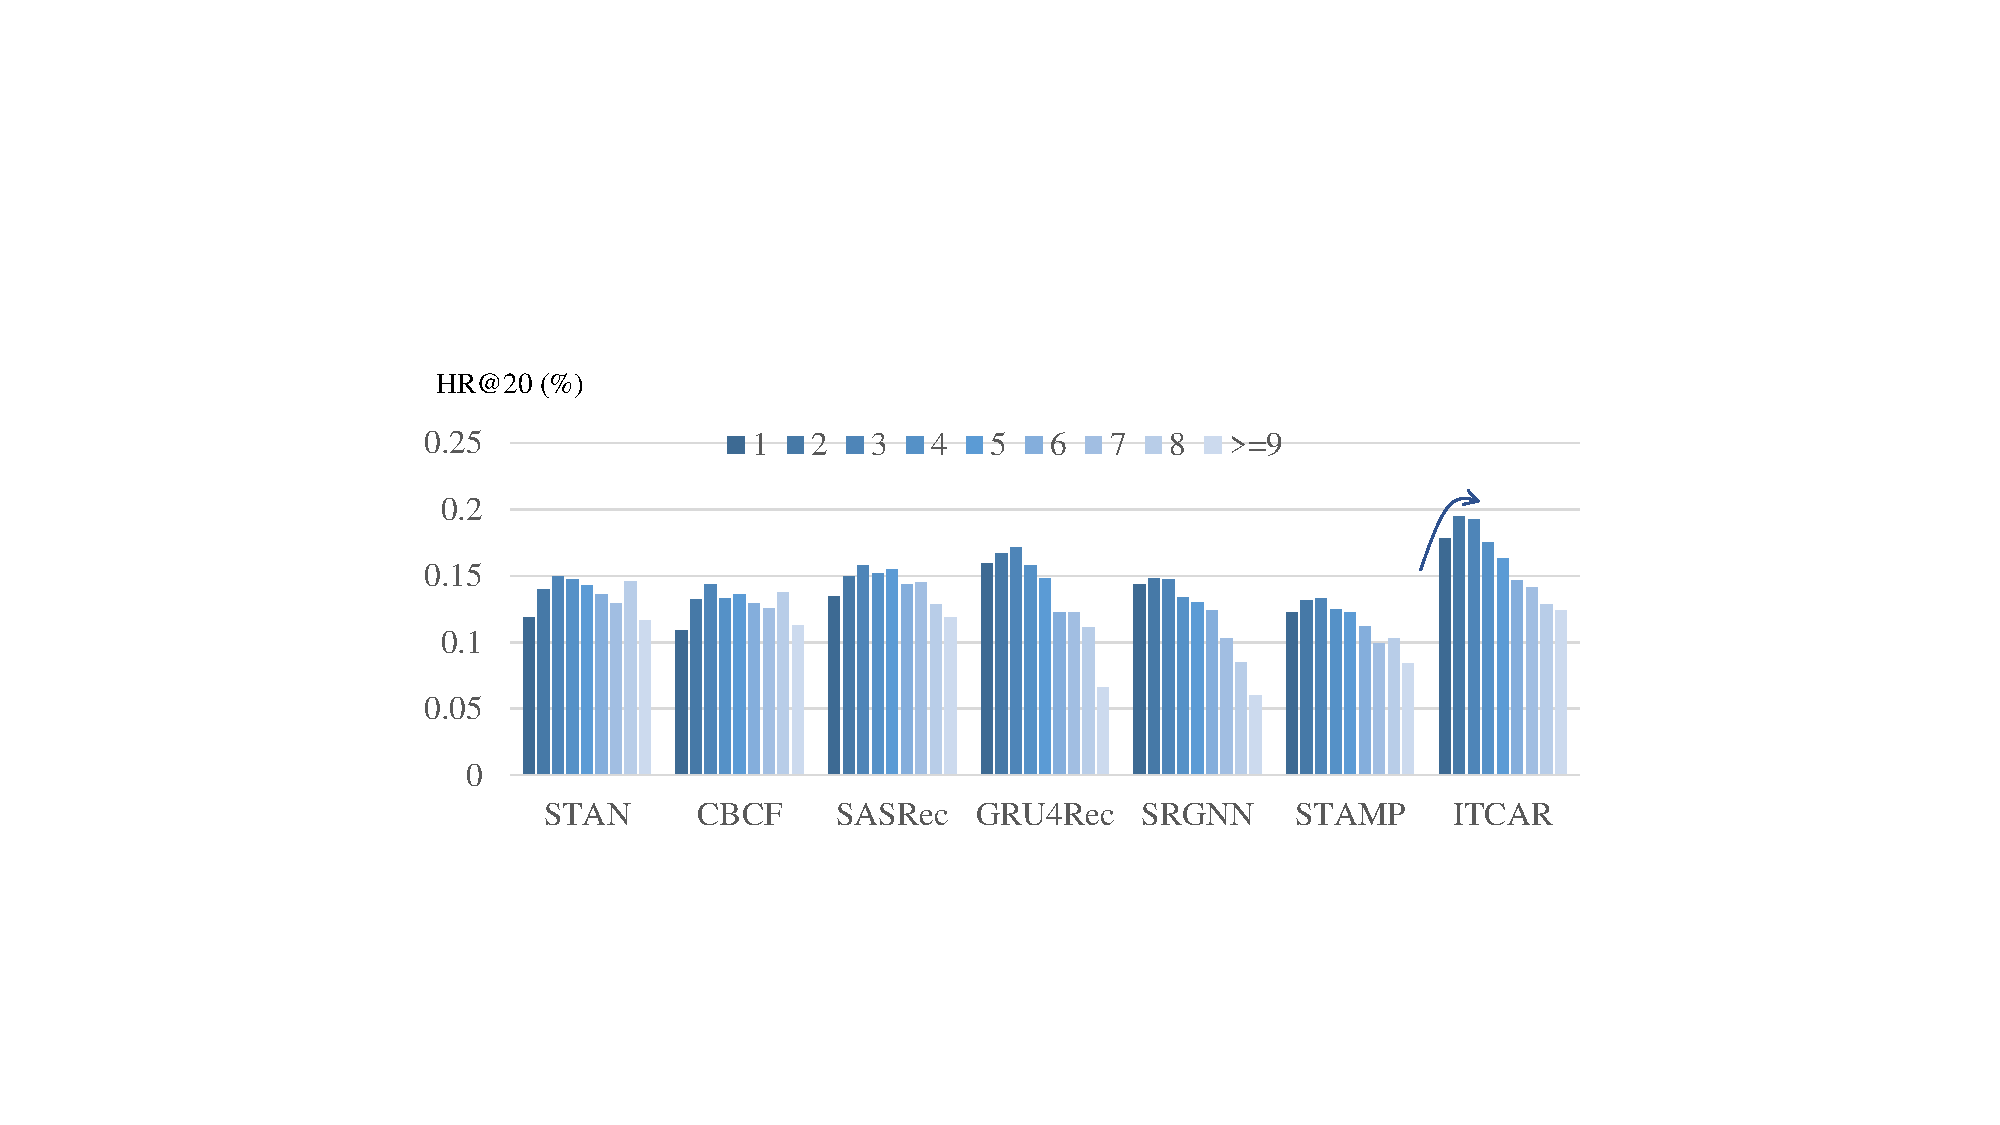
\includegraphics[width=\columnwidth]{fig/input_len.pdf}
  \caption{Accuracy with different session lengths in Globo.}
  \label{fig:inputlen}
  \Description[Results for different input length]{HR@20 results of methods in different length of input.}
\end{figure}

\subsubsection{Article cold-start}
\label{sec:itemcold}
For news recommendation, all methods suffer from article cold-start problem due to the continuously published news, the analyses of the article cold-start scenario can help us 
figure out where our improvement comes from. 
%In the article cold-start situation, none of the articles in input sequence is 
%observed during training, we need to recommend articles based on their content and from the user's implicit feedback. 
\tabref{tb:cold-start} lists the results of all 4 folds in Globo dataset. 
For cold situation, where the test news are completely disjoint from
the training data, STAN does badly because it can't handle unseen items.
Deep learning methods tend to predict the same articles for different users. 
Even though methods like SASRec yields not bad results, 
the models tend to overfit to popular articles. ITCAR, on the other hand, not only performs well on HR@20 but also get the comparable DR@20 score, and the difference with the
other deep learning methods is remarkable. 
\textbf{Cont} model only uses the article encoder and 
\textbf{Time} model only uses the temporal encoder. We can conclude that 
the article encoder contributes to the diversity while the temporal encoder contributes 
to the accuracy in the cold scenarios. 
In non-cold situation, the performance of all methods are close.  
The overall recommendation results largely depends on how a method does for 
cold-start scenarios.

% \begin{table}[!htp]\setlength{\tabcolsep}{2.5pt}
% \caption{Average cold start performance on Globo dataset.}
% \label{tb:cold-start}
% \centering
% \begin{tabular}{c|c|c|c|c|c|c}
%   \toprule
%   \multirow{2}{*}{Methods}  & \multicolumn{2}{c|}{Cold(80.3\%)} & \multicolumn{2}{c|}{non-Cold(19.7\%)} & \multicolumn{2}{c}{Total} \\ \cline{2-7} 
%     & HR@20 & DR@20 & HR@20 & DR@20 & HR@20 & DR@20    \\ 
%   \midrule
%   CBCF & 3.69   & 5.06  &  24.88 & 5.54 & 7.87  & 3.95 \\
%   STAN & -  & - &  26.52  &  1.63 & 5.22   & 0.93  \\ 
%   \midrule
%   GRU4Rec & 1.51  & 0.03  & 20.93 & 0.88 &  5.33  & 0.50 \\
%   SASRec & 0.8  & 0.01  & 23.35 & 1.28 & 5.25 & 0.73 \\
%   SR-GNN & 1.00  & 0.01  &  23.65  & 0.99  & 5.46  & 0.57\\ 
%   STAMP & 1.72 & 0.01 & 21.84  & 1.04 & 5.68 & 0.59 \\
%   \midrule
%   ITCAR & 4.96 & 0.74 & 25.27  & 1.87  & 8.96  & 1.20  \\
%   \bottomrule
% \end{tabular}
% \end{table}

\begin{table}[th]\setlength{\tabcolsep}{2.4pt}
\caption{Article cold-start performance on all of Globo.}
\label{tb:cold-start}
\centering
\begin{tabular}{c|c|c|c|c|c|c}
 \toprule
 \multirow{2}{*}{Methods}  & \multicolumn{2}{c|}{Cold(80.3\%)} & \multicolumn{2}{c|}{non-Cold(19.7\%)} & \multicolumn{2}{c}{Total} \\ \cline{2-7} 
   & HR@20 & DR@20 & HR@20 & DR@20 & HR@20 & DR@20    \\ 
 \midrule
 CBCF & 2.93  & \textbf{5.88}  & 28.11 & \textbf{5.56} & 11.85 & \textbf{4.37} \\
 STAN & -  & - &  \textbf{35.45}  & 1.56 & 12.73  &  0.98  \\ 
 \midrule
 GRU4Rec & 3.09  & 0.04  & 29.05 & 0.55 & 12.80 & 0.35 \\
 SASRec & 3.27 & 0.01  & 33.05 & 1.42 & 14.09 & 0.90 \\
 SR-GNN & 1.72 & 0.01  & 32.15  & 1.08 & 12.64 & 0.68 \\ 
 STAMP & 2.08 & 0.01 & 30.39 & 1.01 & 12.47 & 0.63  \\
 \midrule
 ITCAR & \textbf{9.09} & 0.96 & 34.35 & 1.63 & \textbf{17.87} & 1.48 \\
 Cont & 1.26 & 1.40 & 32.22 & 1.78 & 12.49 & 1.38 \\
 Time & 3.16 & 1.00 & 5.89 & 1.56 & 4.20 & 1.09 \\
 \bottomrule
\end{tabular}
\end{table}

\subsubsection{Different number of days for training/test}
\label{sec:robo}
The result is shown in \figref{fig:trainlen}, and all five folds use the same set of 
test data for fair comparison. The overall performance of ITCAR is consistently 
better with large margins than all other methods regardless the number of training days. 
Most other methods heavily rely on the freshness of items and they generally 
do better closer training data. When we use training data just one day apart from 
the test day, the article cold-start ratio is already extremely high, 
which again shows the fast changing nature of news articles. 
In this situation, ITCAR stands second, only after CBCF,
which does particularly well with its strong focus on content similarity. 

\begin{figure}[th]
  \centering
  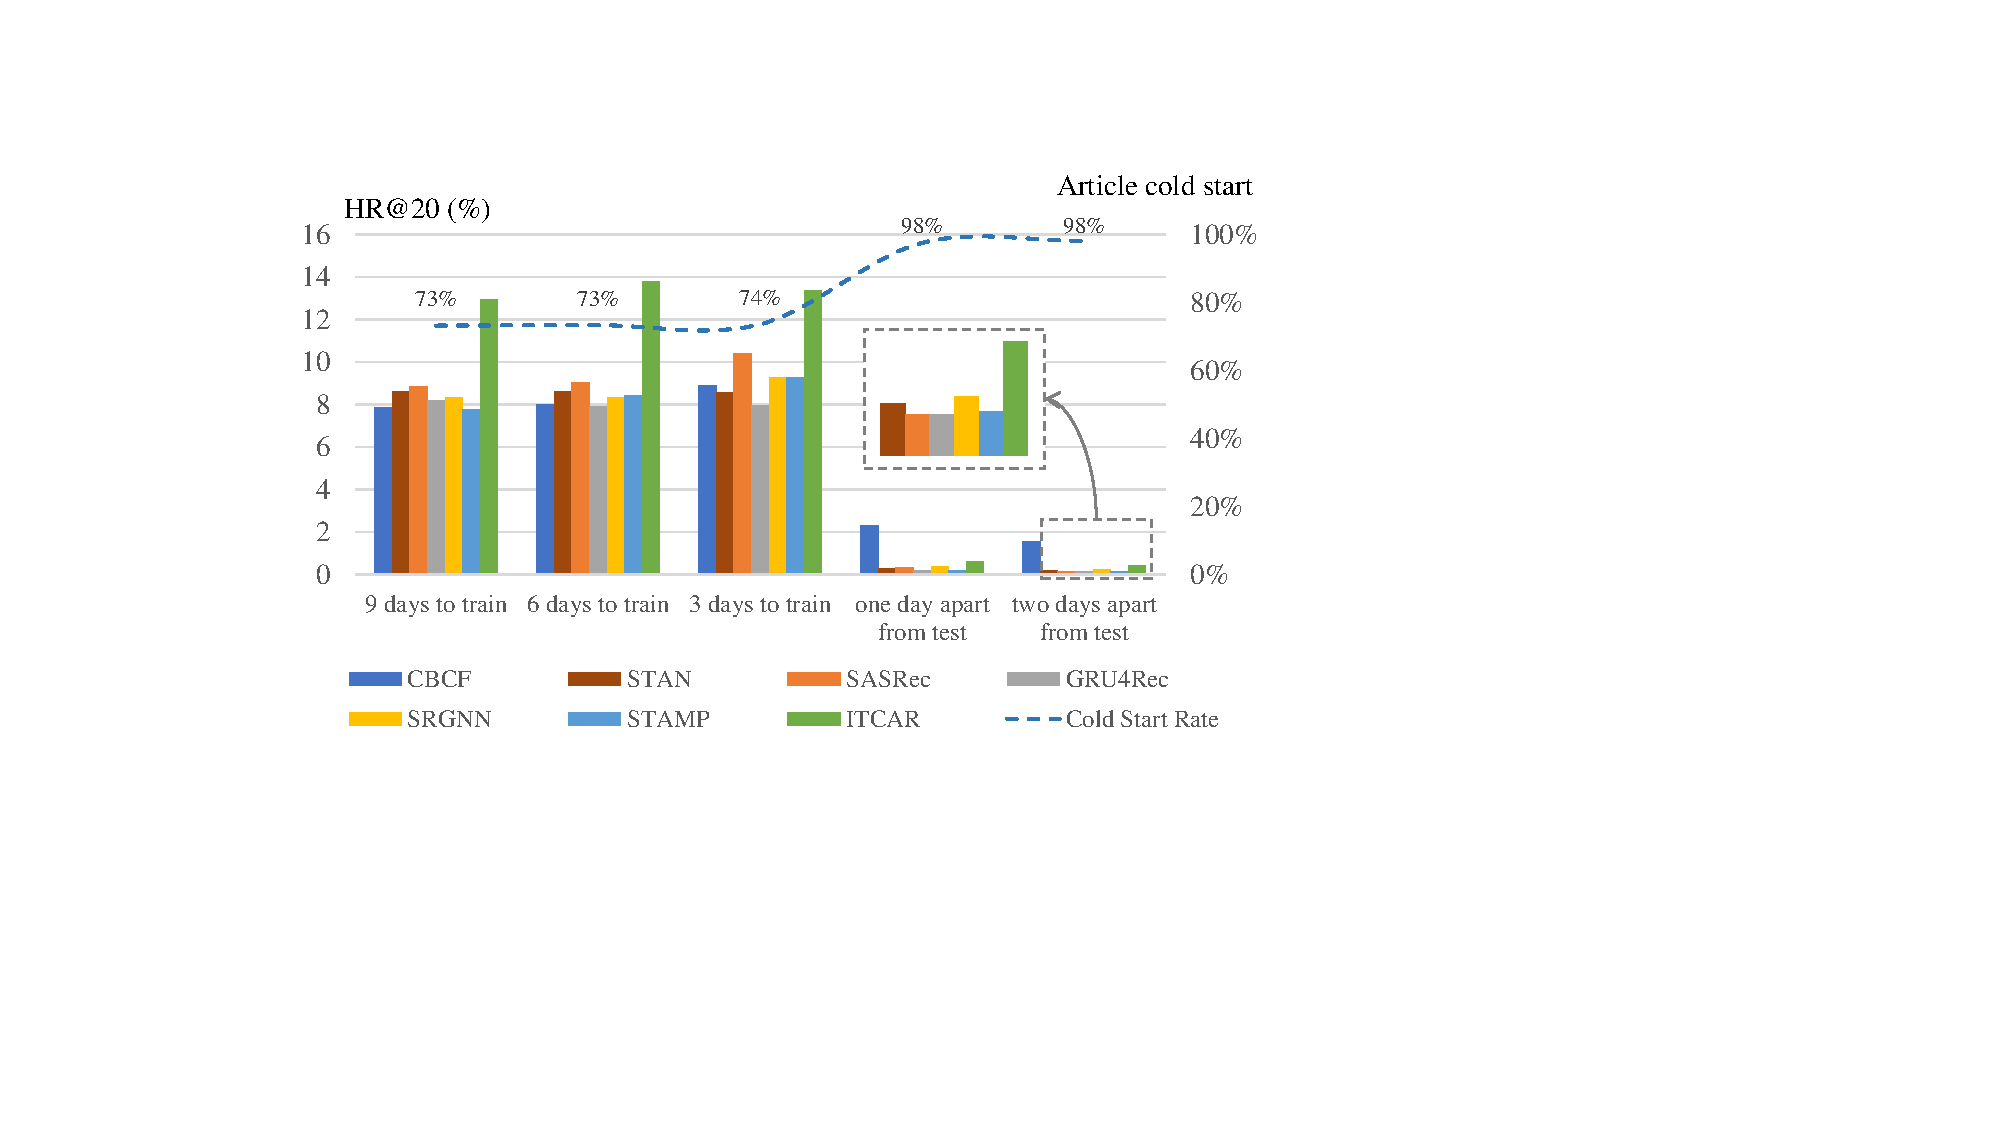
\includegraphics[width=\columnwidth]{fig/diff_day_len.pdf}
  \caption{Accuracy under different train/test splits.}
  \label{fig:trainlen}
\end{figure}

\subsubsection{Inferring user impressions from user clicks}
In this section, we validate our assumption for the negative user feedback,
which is articles whose publish time is close to the clicked articles are
likely presented to the user, or within their impressions.
We do that with the MIND dataset, in which the real impressions, click times and 
publish times of articles are all available for all the sessions. 
We compute the span of the publish times of all the articles in
each session's impression list, including those articles that are clicked. 
We call this \textit{impression time span}.
We find that 63\% of the sessions in MIND have an impression time span of under
one hour. Only 23\% of the sessions have an impression time span of over 12 hours.
This shows that users typically only browse news articles that are created within a small 
time window and click some of them.

